\documentclass[04.3_buildingProcess.tex]{subfiles}
\begin{document}
    \subsubsection{Milling Process}
    \begin{flushleft}
        To build the prototype, we modeled the base for the lamp (see Figure ~\ref{fig:blossomBaseModel}). 
        Therefore, we used Autodesk Fusion 360 \cite{autodeskFusion360}. After designing the base, we used a 
        milling machine. Therefore, we only had to convert the 3D model into a ".iges"-file.
        The result of the milling process can be seen in Figure ~\ref{fig:blossomBase}.

        \begin{figure}[H]
            \centering
            \begin{subfigure}{.45\textwidth}
                \centering
                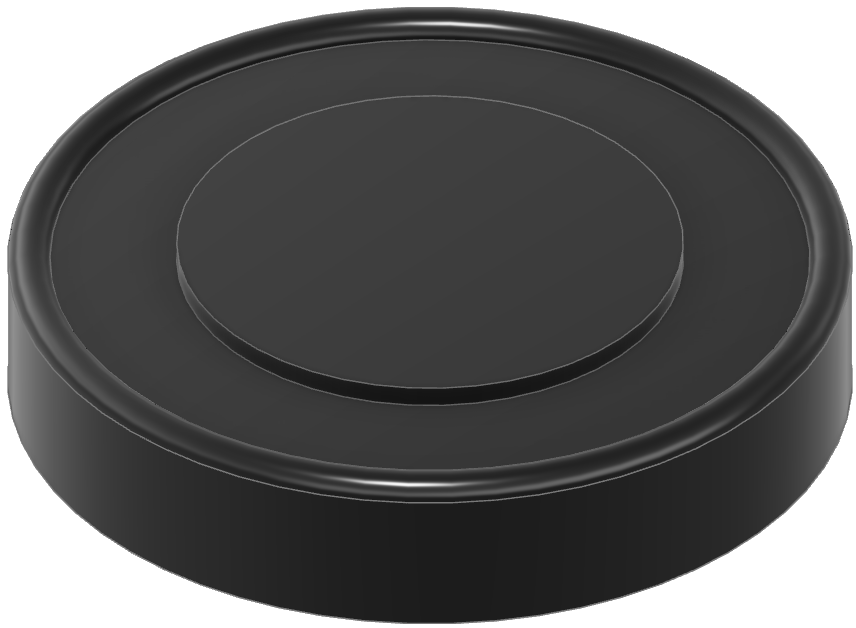
\includegraphics[scale=0.25]{images/materialProcess/FlowerLamp.png}
                \caption{Shows the three-dimensional digital base of the blossom lamp idea.}
                \label{fig:blossomBaseModel}
                \vspace{6mm}
            \end{subfigure}
            \hspace{1mm}
            \begin{subfigure}{.45\textwidth}
                \centering
                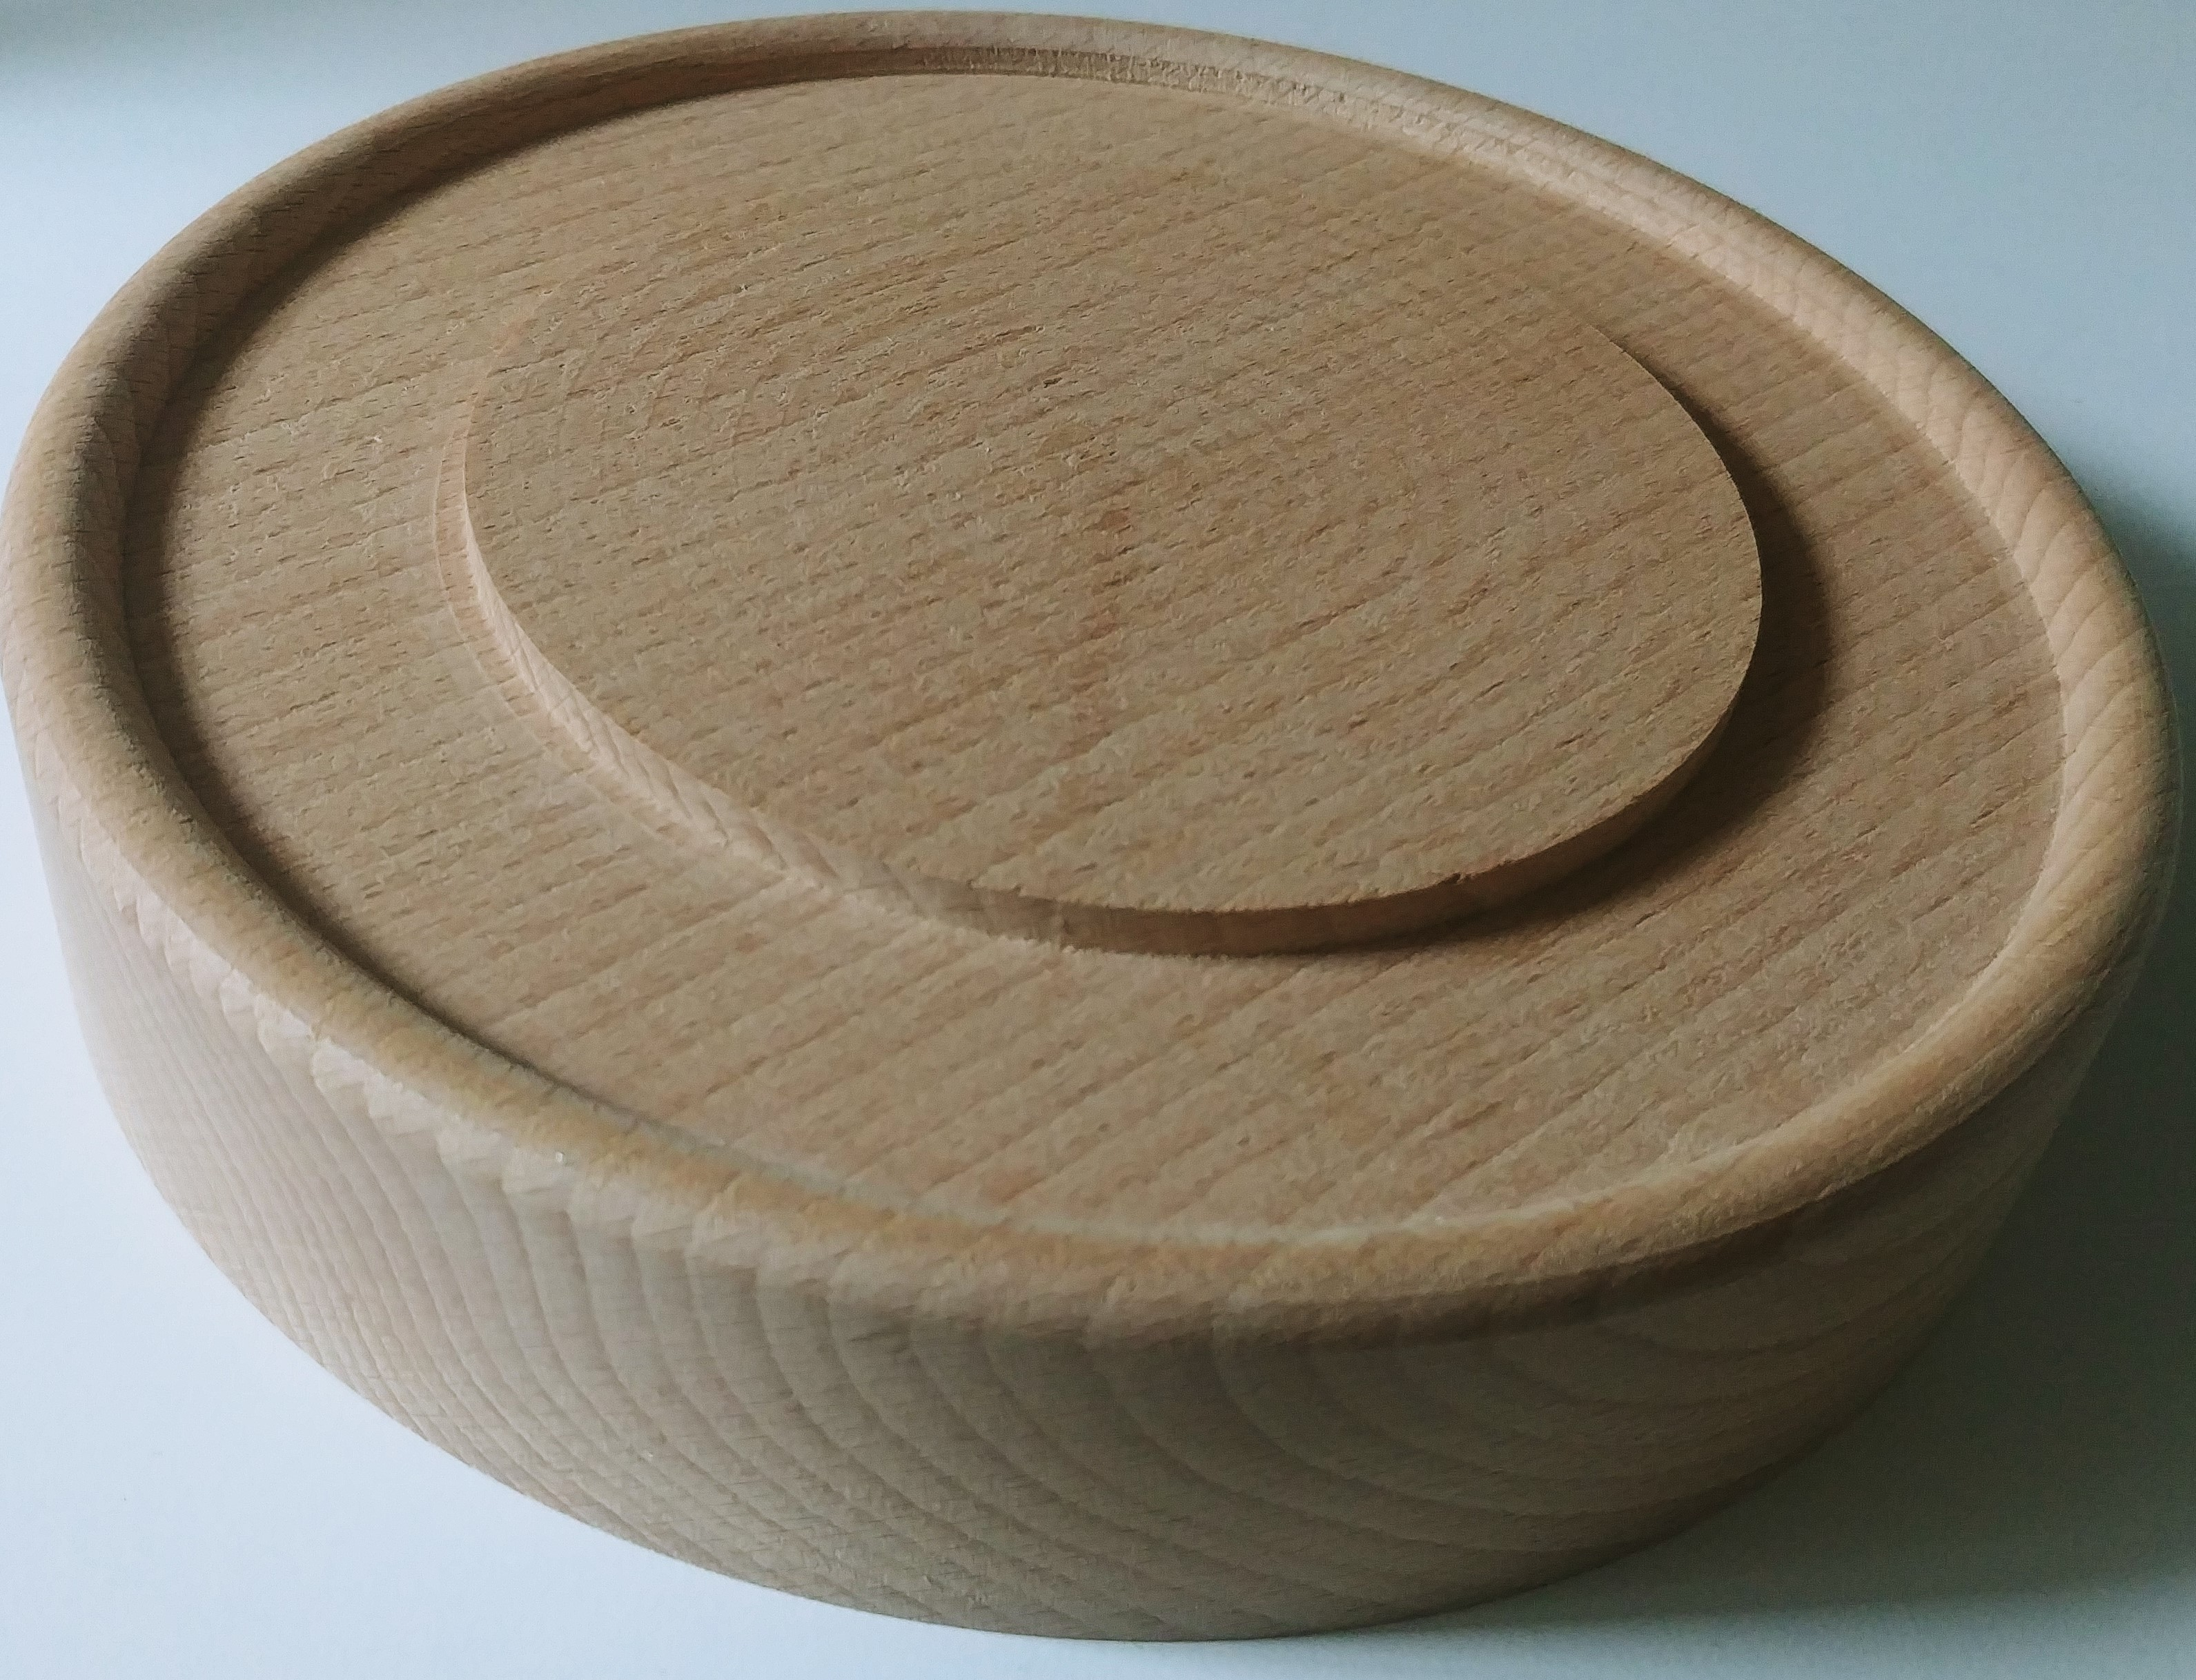
\includegraphics[scale=0.05]{images/materialProcess/base.jpg}
                \caption{Shows the base that has been milled.}
                \label{fig:blossomBase}
                \vspace{6mm}
            \end{subfigure}
            \caption{Show the steps we had to do to drill the base in a CNC machine.}
            \label{fig:laserCutTests}
        \end{figure}
    \end{flushleft}
\end{document}